\chapter{Desenvolvimento}

Este capítulo mostra as decisões e os artefatos produzidos para o desenvolvimento do projeto.
É discutido o suporte tecnológico, a arquitetura do sistema, a representação visual, diagramas, o projeto de dados, a estratégia de testes de software e a prototipação de alta fidelidade.

\section{Suporte Tecnológico}

Esta seção apresenta as ferramentas usadas nesta etapa do trabalho de conclusão de curso assim como as ferramentas planejadas para o desenvolvimento do software na segunda etapa do projeto.
As ferramentas foram escolhidas visando a metodologia ágil do desenvolvimento do MVP e a experiência prévia com as mesmas.

\subsection{Miro}

A ferramenta Miro permite criar diagramas ilustrativos e exportá-los em imagens.
Além disso, a aplicação da metodologia Lean Inception exige um ambiente altamente colaborativo para a construção de artefatos como o Canvas MVP.
O Miro foi utilizado para ilustrar os processos do Lean Inception, facilitando a visualização do produto e o alinhamento das expectativas.

\subsection{Figma}

O Figma é a ferramenta escolhida para a elaboração dos protótipos de alta fidelidade.
Sua relevância está na capacidade de criar componentes reutilizáveis e fluxos de interação que simulam a experiência real do usuário.
Portanto, o Figma é útil para validar a interface e testar a usabilidade das funcionalidades antes da codificação \cite{figma_2025}.

\subsection{Draw.io}

O Draw.io foi utilizado para a modelagem dos diagramas de classe e diagramas de pacotes.
A ferramenta permite documentar a arquitetura lógica do aplicativo, essencial para garantir que a integração entre os componentes e o banco de dados seja implementada de forma correta \cite{drawio_2025}.

\subsection{React Native e Expo}

Para o desenvolvimento, planeja-se o uso do React Native junto com o framework Expo.
Essa escolha justifica-se pela necessidade de uma aplicação mobile (Android) que utilize uma base de código única.
O Expo acelera o desenvolvimento ao fornecer APIs prontas para notificações e acesso ao hardware, além de permitir testes em tempo real em dispositivos físicos através do Expo Go \cite{expo_2025}.

\subsection{Node.js e Express}

Como tecnologia de backend, planeja-se a utilização do Node.js com o framework Express.
Este conjunto tecnológico é reconhecido pela sua escalabilidade e alta performance em aplicações com bancos de dados, sendo ideal para gerenciar as requisições de check-ins de saúde e o processamento do algoritmo de repetição espaçada em tempo real.

\subsection{PostgreSQL}

Para a persistência dos dados, planeja-se usar o PostgreSQL como o Sistema Gerenciador de Banco de Dados Relacional do aplicativo.
Suportando consultas complexas e garantindo a integridade conforme as normas da LGPD.

\subsection{Git e GitHub}

O controle de versionamento do código será realizado utilizando Git, com o armazenamento dos repositórios no GitHub.
Essa prática é ideal para a manutenção do histórico do código, permitindo o gerenciamento de ramos para novas funcionalidades e assegurando a segurança e integridade do código durante o ciclo de desenvolvimento \cite{github_2025}.

\subsection{Trello}

Para o gerenciamento ágil do projeto, o Trello será utilizado como a ferramenta do quadro do Kanban.
Ele permitirá o acompanhamento das tarefas elicitadas no Sequenciador do Lean Inception, facilitando a organização das sprints de desenvolvimento e a visualização do progresso das features do MVP em tempo real.

\subsection{SonarQube}

O SonarQube será utilizado para a análise estática de código, permitindo identificar bugs e vulnerabilidades.
Como destacam \citeonline{gobov_2025}, garantir atributos de qualidade como manutenibilidade e confiabilidade é crucial.
O uso do SonarQube reduz o risco e assegura um software mais confiável \cite{sonarsource_2025}.

\subsection{BrModelo}

A ferramenta BrModelo foi utilizada para fazer o projeto de dados (diagrama entidade-relacionamento e diagrama lógico de dados).
Através dessa ferramenta, realiza-se a modelagem conceitual e lógica do sistema.

\section{Arquitetura}

Segundo \citeonline{dipompeo_2025}, a arquitetura é uma abstração de alto nível que funciona como um guia para a implementação, sendo essencial para os aspectos de qualidade, como performance, confiabilidade e manutenibilidade.
Dessa forma, o modelo adotado busca equilibrar as necessidades de negócio e os objetivos técnicos do sistema. Foi definido que o modelo Arquitetural em Camadas será seguido no desenvolvimento.

\subsection{Padrão Arquitetural em Camadas}

A definição da estrutura arquitetural visa mitigar riscos.
Conforme destacado por \citeonline{khalid_2025}, a má gestão de requisitos e de sua tradução técnica é uma causa primária de falhas em projetos.
Para evitar esse cenário, adotou-se uma organização em camadas que isola as preocupações de interface, lógica de negócio e persistência de dados.

Esta separação permite que a arquitetura facilite a evolução do código sem comprometer a estabilidade do sistema \cite{dipompeo_2025}.
As camadas são divididas em:

\begin{itemize}
    \item \textbf{Apresentação (View):} Interface móvel que interage com o usuário.
    \item \textbf{Processamento (Controller/Service):} Onde as funções são validadas e executadas.
    \item \textbf{Acesso a Dados (Repository/Model):} Camada que abstrai a complexidade do banco de dados relacional.
\end{itemize}

\subsection{Backend}

O backend, desenvolvido em Node.js, atua como o núcleo da aplicação.
De acordo com \citeonline{dipompeo_2025}, a especificação cuidadosa do design arquitetural permite fortalecer a confiabilidade do software.
Dessa forma, a lógica de agendamento de revisões e os cálculos são centralizados no servidor para garantir a integridade dos dados e o cumprimento dos requisitos de qualidade.

A organização interna do backend será estruturada para suportar atributos de qualidade como a manutenibilidade, distribuindo as responsabilidades da seguinte forma:

\begin{itemize}
    \item \textbf{Controllers:} Responsáveis por receber e responder às requisições da interface.
    \item \textbf{Services:} Camada onde reside a lógica de domínio, isolada de interferências externas.
    \item \textbf{Repositories:} Camada dedicada exclusivamente à interação com o SGBDR PostgreSQL.
\end{itemize}

\subsection{API RESTful e Segurança}

A comunicação entre o cliente e o servidor será estabelecida através de uma API RESTful baseada no protocolo HTTP e no formato JSON.
Essa escolha agrega performance conforme preconizado por \citeonline{gobov_2025} ao discutirem as características de eficiência de tempo.
Para assegurar a confidencialidade e a integridade das informações dos usuários, a arquitetura implementará autenticação via JSON Web Token, alinhando-se às boas práticas de segurança mencionadas por \citeonline{dipompeo_2025} como técnicas para preservação da qualidade arquitetural.

\subsection{Mapeamento Objeto-Relacional (ORM)}

Para garantir a qualidade na persistência dos dados, utilizará um mapeamento objeto-relacional (ORM) que faz a ligação entre o Node.js e o PostgreSQL.
Essa camada de abstração é útil para a manutenção, pois permite que a estrutura do banco de dados evolua com baixo impacto na camada de serviços.
Além disso, o uso do ORM facilita a implementação dos requisitos técnicos.

\subsection{Frontend}

O frontend representa a interface do sistema e deve satisfazer os atributos de usabilidade e experiência do usuário.
Segundo \citeonline{gobov_2025}, a usabilidade é um atributo de qualidade externo que determina quanto o usuário final consegue operar a ferramenta.
Portanto, a arquitetura do frontend foi desenhada para ser intuitiva, reduzindo a dificuldade do usuário durante o uso.

\subsubsection{React Native e Expo}

A escolha do React Native como base tecnológica permite a criação de componentes de software reutilizáveis, cujas propriedades e relacionamentos definem a dinâmica da interface.
A utilização do framework Expo complementa essa estrutura ao facilitar o acesso a recursos nativos do hardware do dispositivo.
Essa abordagem assegura que a qualidade do software, conforme definida por \citeonline{khalid_2025}, seja mantida independentemente do sistema Android utilizado pelo usuário, otimizando o processo de entrega de valor.

\section{Representação Visual do Sistema}

A representação visual do sistema constitui na implementação da arquitetura proposta, traduzindo abstrações conceituais em diagramas técnicos que orientam o desenvolvimento, a fim de gerenciar a complexidade do software.
Através de modelos visuais, busca-se estabelecer um modelo que assegura a integridade entre os requisitos de software e a estrutura física do código, garantindo que os atributos de qualidade sejam preservados durante todo o ciclo de vida.

\subsection{Diagrama de Classes}

O Diagrama de Classes do sistema foi estruturado para definir as entidades fundamentais, seus atributos e seus relacionamentos de dependência.
De acordo com a pesquisa de \citeonline{kim_2024}, a eficácia de um diagrama de classe está diretamente ligada ao seu layout e controle de complexidade, uma vez que esses fatores impactam significativamente a compreensibilidade do modelo pelo desenvolvedor.
Para garantir isso, o diagrama foi organizado seguindo um fluxo lógico de leitura, a seguir está representado o diagrama de classes deste projeto.

\begin{figure}[H]
    \centering
    \caption{Diagrama de Classes}
    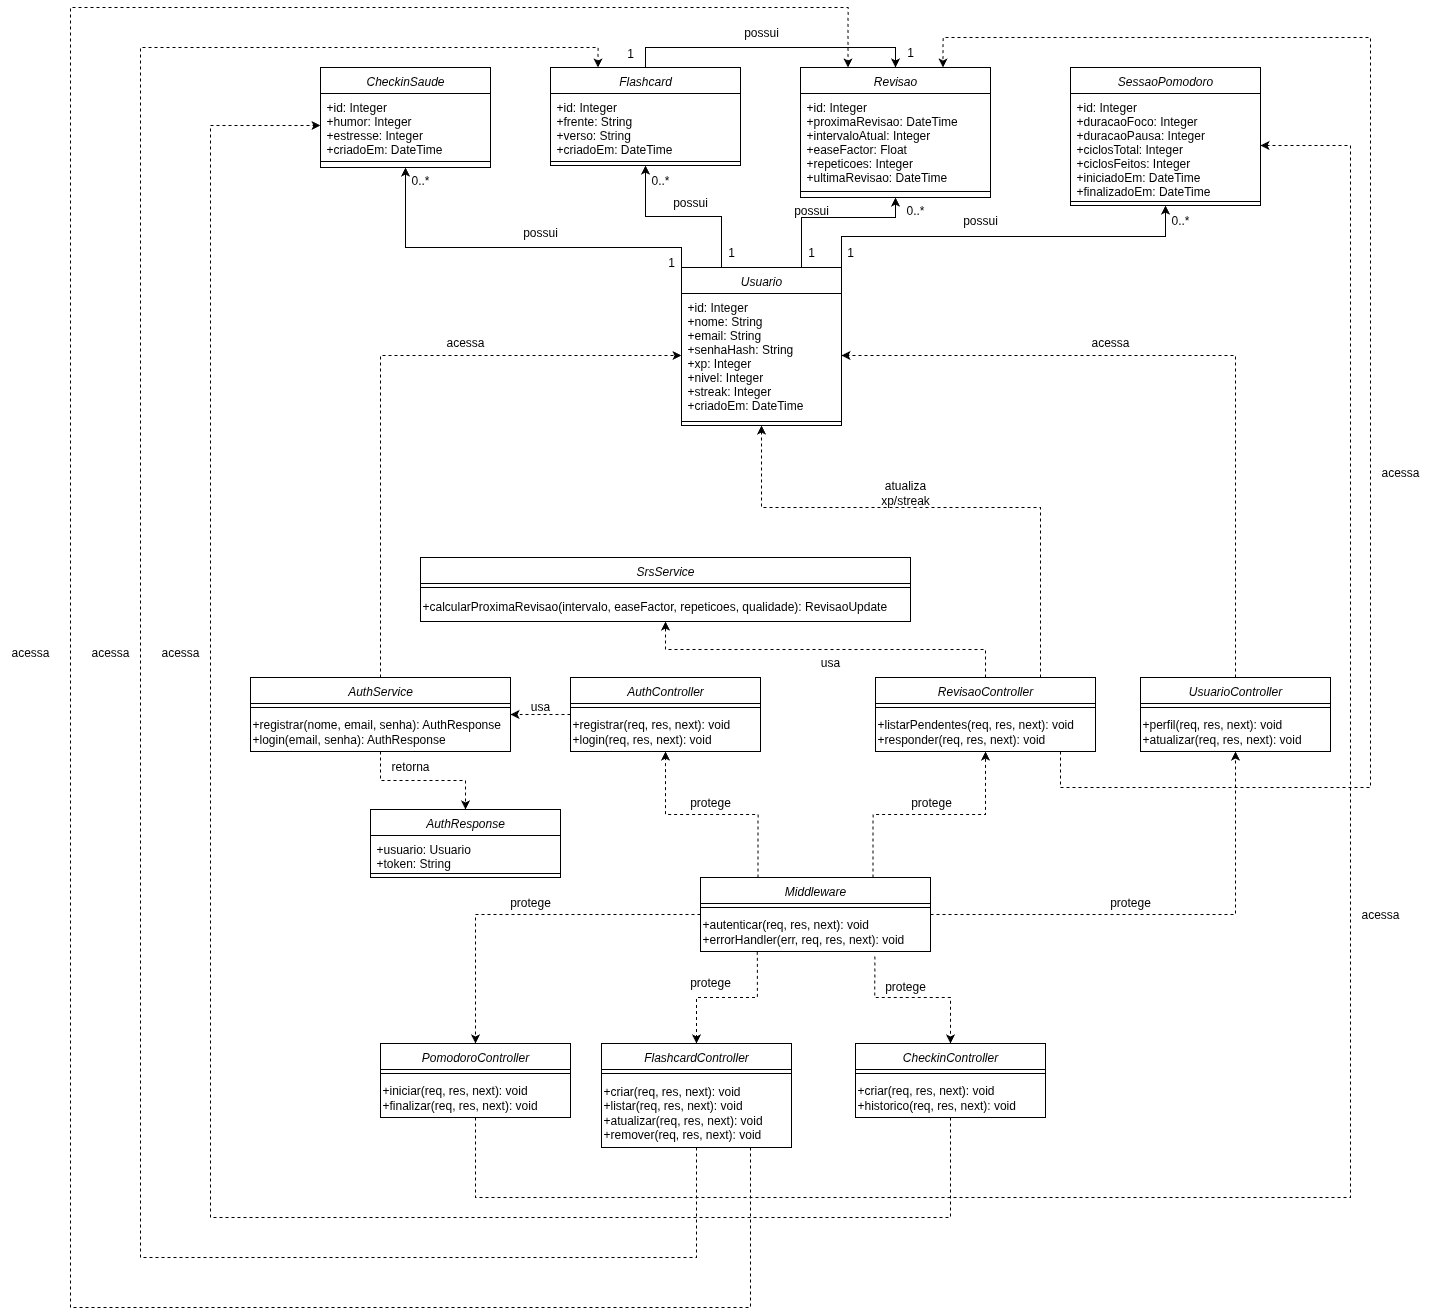
\includegraphics[width=1\linewidth]{Imagens/DiagramaClasses.drawio.png}
    \par
    Fonte: Autoria própria.
    \par
    \label{fig:diagrama_classes}
\end{figure}

\subsection{Diagrama de Pacotes}

Os Diagramas de Pacotes organizam os elementos do sistema em módulos lógicos, isolando as necessidades do frontend e do backend.
No frontend, a segmentação em pacotes de interface, lógica e serviços visa maximizar a manutenibilidade e a usabilidade \cite{gobov_2025}.
No backend, a estruturação em camadas de rotas, controladores e serviços reflete o compromisso com o baixo acoplamento e a confiabilidade.
Essa organização visual é essencial para mitigar falhas na tradução dos requisitos \cite{khalid_2025}, permitindo que cada pacote evolua de forma independente sem comprometer a estabilidade do aplicativo.
A seguir estão representados os diagramas de pacotes deste trabalho.

\begin{figure}[H]
    \centering
    \caption{Diagrama de Pacotes do Backend}
    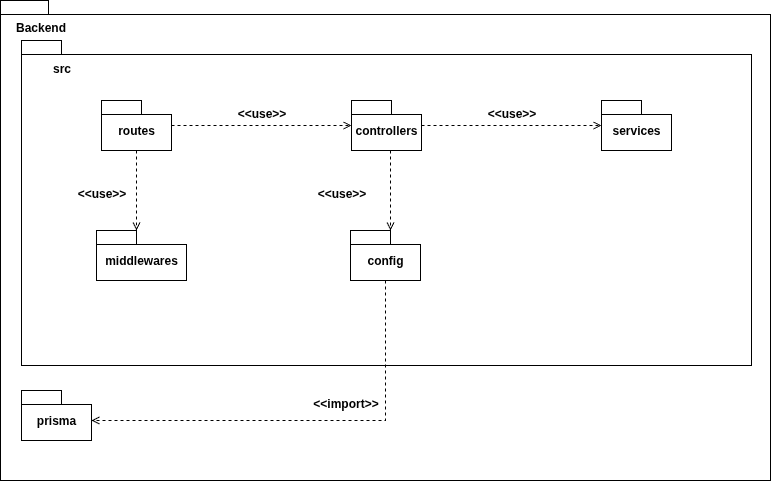
\includegraphics[width=1\linewidth]{Imagens/DiagramaPacotesBackend.png}
    \par
    Fonte: Autoria própria.
    \par
    \label{fig:diagrama_pacotes_backend}
\end{figure}

\begin{figure}[H]
    \centering
    \caption{Diagrama de Pacotes do Frontend}
    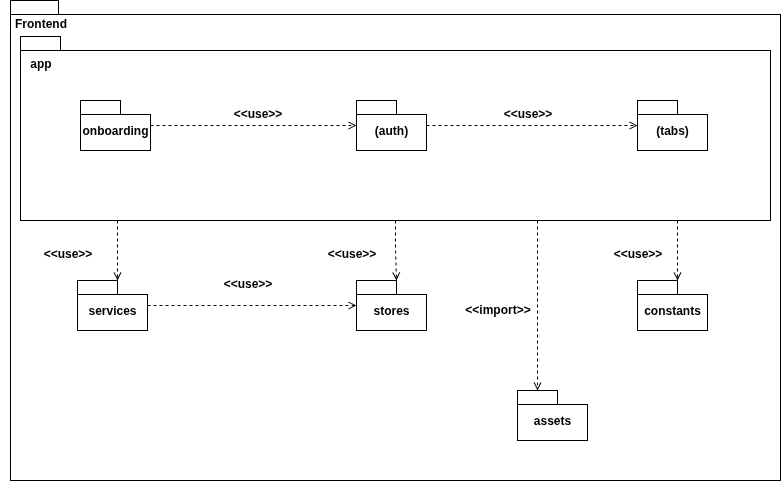
\includegraphics[width=1\linewidth]{Imagens/DiagramaPacotesFrontend.png}
    \par
    Fonte: Autoria própria.
    \par
    \label{fig:diagrama_pacotes_frontend}
\end{figure}

\section{Projeto de Dados}

O Projeto de Dados tem como objetivo modelar a estrutura de persistência dos dados do aplicativo, definindo as entidades, atributos e relacionamentos do mesmo.
A modelagem foi realizada em dois níveis: o Diagrama Entidade-Relacionamento, que representa de forma abstrata as entidades e seus relacionamentos, e o Diagrama Lógico, que traduz essa abstração em uma estrutura compatível com o Sistema Gerenciador de Banco de Dados Relacional.
Todas decisões de modelagem foram guiadas pelos requisitos funcionais e não funcionais levantados anteriormente.

\subsection{Diagrama Conceitual}

A etapa conceitual da modelagem de dados é responsável por abstrair as entidades do sistema, seus atributos e os relacionamentos existentes entre elas, de forma universal e compatível com qualquer tecnologia de banco de dados através do Diagrama Entidade-Relacionamento (DE-R).
Essa etapa exige a transformação dos requisitos em um modelo com regras, envolvendo uma abstração maior do que nas próximas etapas, sendo apontada como a principal fonte de dificuldades cognitivas no processo de modelagem \cite{shin_2025}.
Para este trabalho, o DE-R foi construído a partir das entidades identificadas durante o Lean Inception e o levantamento de requisitos.
A seguir está representado o DE-R deste projeto.

\begin{figure}[H]
    \centering
    \caption{Diagrama Entidade-Relacionamento (DE-R) do Projeto}
    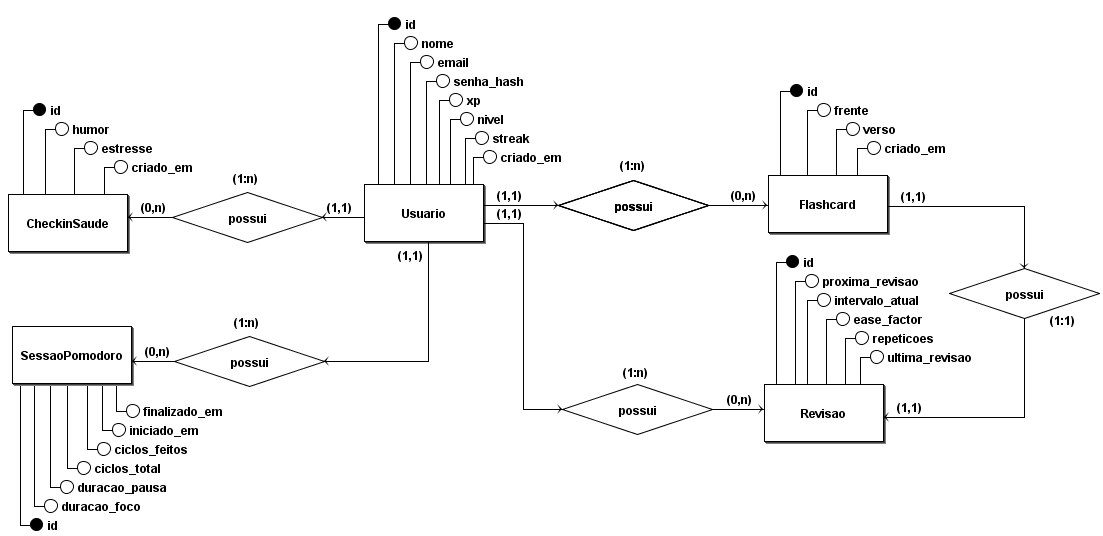
\includegraphics[width=1\linewidth]{Imagens/DiagramaConceitual.png}
    \par
    Fonte: Autoria própria.
    \par
    \label{fig:diagrama_conceitual}
\end{figure}

\subsection{Diagrama Lógico}

Já o Diagrama Lógico representa a segunda etapa da modelagem de dados, sendo responsável por transformar a abstração do DE-R em uma estrutura lógica compatível com o modelo relacional, definindo tabelas, colunas, chaves primárias, chaves estrangeiras e as restrições de integridade referencial entre as entidades.
Essa transição do modelo conceitual para o modelo lógico segue um conjunto de regras de mapeamento bem definidas, onde cada entidade do diagrama conceitual é transformada em uma tabela, cada atributo em uma coluna e cada relacionamento em uma chave estrangeira alocada no lado correto da cardinalidade ou em uma nova relação.
Esse processo de mudança do modelo entre níveis de abstração é um dos pilares do desenvolvimento orientado a modelos, no qual modelos universais são aperfeiçoados em modelos mais específicos por meio de regras de mapeamento \cite{lo_2012}.
Para este trabalho, o Diagrama Lógico foi derivado diretamente do DE-R, respeitando as cardinalidades levantadas e as decisões de modelagem tomadas durante o Lean Inception, resultando em um esquema relacional normalizado, pronto para ser implementado no SGBD.
A seguir está representado o Diagrama Lógico deste projeto.

\begin{figure}[H]
    \centering
    \caption{Diagrama Lógico do Projeto}
    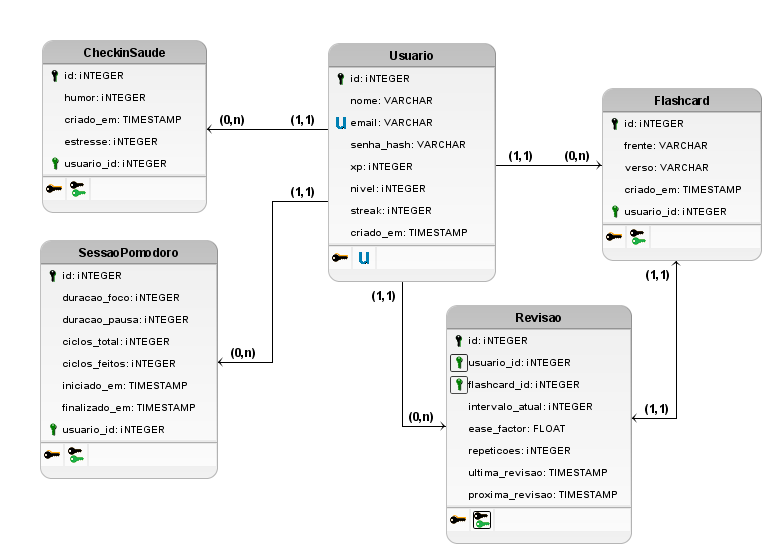
\includegraphics[width=1\linewidth]{Imagens/DiagramaLogico.png}
    \par
    Fonte: Autoria própria.
    \par
    \label{fig:diagrama_logico}
\end{figure}

\section{Testes de Software}

A etapa de testes faz parte do ciclo de vida de desenvolvimento do software, sendo definido como o processo que engloba todas as atividades do ciclo de vida, estáticas e dinâmicas, relacionadas ao planejamento, preparação e avaliação do mesmo, com o objetivo de verificar se satisfaz os requisitos especificados, demonstrar que estão aptos para o uso e detectar defeitos \cite{goericke_2020}.
A falta dessa etapa representa um risco ao projeto, pois bugs são significativamente mais fáceis e baratos de corrigir em estágios iniciais do desenvolvimento do que em fases avançadas ou após a entrega ao usuário final \cite{goericke_2020}.

O desenvolvimento deste projeto adota a prática de TDD como estratégia de qualidade, que desempenha um papel fundamental na definição da estratégia de testes ao longo de todo o desenvolvimento \cite{goericke_2020}.
O TDD garante que cada módulo do aplicativo, como o algoritmo de repetição espaçada, seja coberto por testes, assegurando que as regras de negócio estejam sempre verificáveis e coerentes aos requisitos.

A estratégia de testes adotada segue a pirâmide de testes, que divide os testes em três: os testes unitários, que podem ser executados em níveis unitários, os testes de integração que são mais lentos pois integram dois ou mais módulos e os testes de sistema que englobam todo o sistema.
Dessa forma, os testes unitários, níveis mais baixos, são os mais adequados para automação \cite{goericke_2020}.
Portanto, a base da pirâmide será composta por testes unitários automatizados para cobrir as regras de negócio do backend, seguidos de testes de integração para validar a comunicação entre os módulos e o banco de dados, e testes de sistema para verificar os fluxos em níveis de sistema.

Para aplicações móveis, a quantidade de módulos de qualidade a serem considerados representam o principal desafio dos testes, englobando a funcionalidade, a usabilidade, o desempenho, a segurança, a interoperabilidade e a confiabilidade \cite{goericke_2020}.
Diante disso, apesar do aplicativo proposto ser desenvolvido para o sistema Android, não será possível cobrir todos os dispositivos e versões existentes.
Portanto, os testes de usabilidade serão realizados em um número limitado de aparelhos Android, priorizando os modelos mais utilizados pelo público.

\section{Prototipação}

A prototipação é a etapa do desenvolvimento onde as interfaces de usuário são modeladas através de um processo de criação de representações visuais.
Essas representações devem mostrar como a interface deve ser e como os usuários devem interagir com ela, com base nos requisitos do software \cite{letaw_2024}.
Essa abordagem oferece uma experimentação da interface e a identificação de problemas recentes.
Logo, alterar um protótipo de alta fidelidade é mais fácil e rápido do que alterar sua implementação em código \cite{letaw_2024}.

Conforme \citeonline{letaw_2024}, existem três níveis de protótipos: o de baixa fidelidade, composto por esboços aproximados que permitem coletar feedback sobre funcionalidades de alto nível com grande flexibilidade para mudanças; o de média fidelidade, uma ilustração mais detalhada que permite coletar feedback sobre pequenas mudanças em funcionalidades já definidas; e o de alta fidelidade, um modelo digital que se assemelha a uma interface pronta, permitindo coletar feedback sobre ajustes específicos.

Para este projeto, foi utilizado o Figma como ferramenta de criação de protótipos de alta fidelidade.
Portanto, os requisitos funcionais foram validados, reduzindo o risco de retrabalho durante a fase de desenvolvimento do código.
O protótipo desenvolvido foi utilizado como base para o desenvolvimento das páginas principais do aplicativo. Essas páginas podem ser vistas no Apêndice~\ref{apendice:prototipo} deste trabalho.
